\documentclass[10pt,t,english]{beamer}
\usepackage{fontawesome}
\usepackage{graphicx}
\usepackage{array}
\usepackage[normalem]{ulem}
\usepackage{amsfonts,amsmath,amssymb,bm,bbm}
\usepackage{mathrsfs}
\usepackage{sgame}
\usepackage{graphicx,pstricks}
\usepackage{xcolor}
\usepackage{colortbl}
\usepackage{makecell}
\usepackage{tikz,tikzsymbols,gnuplottex}
\usetikzlibrary{decorations.pathreplacing,shapes}
\usepackage[english]{babel}
\usepackage[utf8]{inputenc}
\usepackage{appendixnumberbeamer}
\usepackage{datetime2}
\usepackage{booktabs}
\usepackage{setspace}
\usepackage{rotating}
\usepackage{natbib}
\usepackage{listings}

%\usepackage{matlab-prettifier} % For enhanced MATLAB highlighting
\lstset{
    language=matlab,
    % Other options for styling (optional)
    basicstyle=\ttfamily\footnotesize, % Font style
    keywordstyle=\color{blue}, % Keyword color
    commentstyle=\color{green!50!black}, % Comment color
    stringstyle=\color{red!70!black}, % String color
    numbers=left, % Line numbers on the left
    numberstyle=\tiny\color{gray}, % Style for line numbers
    frame=single, % Frame around the listing
    breaklines=true, % Allow line breaking
    captionpos=b, % Caption at the bottom
    tabsize=4 % Tab size
}

% ------------------------------------------------------------------------------
% Use the beautiful metropolis beamer template
% ------------------------------------------------------------------------------
\usepackage[T1]{fontenc}
\usepackage[utf8]{inputenc}
\usepackage{fontawesome}
\usepackage{FiraSans} 
\mode<presentation>
{
  \usetheme[progressbar=foot,background=light]{metropolis} 
  \usecolortheme{default} % or try albatross, beaver, crane, ...
  \usefonttheme{default}  % or try default, serif, structurebold, ...
  \setbeamertemplate{navigation symbols}{}
  \setbeamertemplate{caption}[numbered]
  %\setbeamertemplate{frame footer}{My custom footer}
} 

\newenvironment{stepenumerate}{\begin{enumerate}[<+->]}{\end{enumerate}}
\newenvironment{stepitemize}{\begin{itemize}[<+->]}{\end{itemize} }
\newenvironment{stepenumeratewithalert}{\begin{enumerate}[<+-| alert@+>]}{\end{enumerate}}
\newenvironment{stepitemizewithalert}{\begin{itemize}[<+-| alert@+>]}{\end{itemize} }

\newtheorem{question}{Question}
\newtheorem{claim}{Claim}
\newtheorem{proposition}{Proposition}
\newtheorem{remark}{Remark}
\newtheorem{conjecture}{Conjecture}

\definecolor{metrop}{RGB}{29, 44, 44}
\colorlet{GrayLight}{black!15}
\colorlet{GrayMedium}{black!30}
\colorlet{ForestGreen}{green!60!black}

\newenvironment{transitionframe}{
  \setbeamercolor{background canvas}{bg=black!80}
  \begin{frame}}{
    \end{frame}
}

\newcommand{\br}{

\bigskip

}

\newcommand{\pd}{\partial}
\newcommand{\RR}{\mathbb{R}}

\newcommand*\hugme[1]{\tikz[baseline=(char.base)]{\node[shape=ellipse,draw,inner sep=0pt] (char) {#1};}}

\newcounter{saveenumi}
\newcommand{\seti}{\setcounter{saveenumi}{\value{enumi}}}
\newcommand{\conti}{\setcounter{enumi}{\value{saveenumi}}}
\resetcounteronoverlays{saveenumi}



\newcommand\dotprod[2]{\langle #1 , #2 \rangle}
\newcommand{\ft}[1]{\widehat #1}
\newcommand{\qabove}[1]{\overset{\text{\large \textbf ?}}{#1}}
\newcommand{\eqae}{\overset{\text{a.e.}}{=}}
\newcommand{\calp}{\mathcal{P}}
\newcommand{\calg}{\mathcal{G}}
\newcommand{\calb}{\mathcal{B}}
\newcommand{\textd}{\text{d}}
\newcommand{\bbr}{\mathbb{R}}
\newcommand{\binm}{\mathbin{M}}
\newcommand{\binc}{\mathbin{C}}
\newcommand{\binb}{\mathbin{B}}
\newcommand{\calc}{\mathcal{C}}
\newcommand{\calh}{\mathcal{H}}
\newcommand{\bfone}{\mathbf{1}}
\newcommand{\bbe}{\mathbb{E}}
\newcommand{\bfle}{\mathbf{e}}
\newcommand{\calf}{\mathcal{F}}
\newcommand{\cala}{\mathcal{A}}
\newcommand{\cale}{\mathcal{E}}
\newcommand{\bbn}{\mathbb{N}}
\newcommand{\cantor}{\calc}
\newcommand{\calY}{\mathcal{Y}}
\newcommand{\textb}{\text{B}}
\newcommand{\calm}{\mathcal{M}}
\newcommand{\bint}{\mathbin{T}}
\newcommand{\ep}{\epsilon}
\newcommand{\bbq}{\mathbb{Q}}
\newcommand{\bbp}{\mathbb{P}}
\newcommand{\cals}{\mathcal{S}}
\newcommand{\emptysequence}{e}
\newcommand{\bbz}{\mathbb{Z}}
\newcommand{\fraka}{\frak{A}}
\newcommand{\frakb}{\frak{B}}
\newcommand{\length}{\text{length}}
\newcommand{\bfn}{\mathbf{N}}
\newcommand{\support}{\text{support}}
\DeclareMathOperator*{\argmax}{arg\,max}
\newcommand{\dom}{\mbox{dom}}
\def\ut{\underline t}
\def\um{\underline m}
\def\PP{\mathbb{P}}
\def\EE{\mathbb{E}}
\def\RR{\mathbb{R}}

\begin{document}

% Title page info
\title[Incentives in Experiments: Theory]{ExpEcon Methods:\\A Theory of Testing Theories}
\author[ECON 8877]{ECON 8877\\P.J. Healy} \color{metrop}
\institute[OSU]{}
\date[]{\vfill {\tiny Updated \today\ at\ \DTMcurrenttime}} % Full_Date\\Location

\frame{\maketitle}

\begin{frame}{Introduction}{}
A principal wants to learn \emph{something} about the preferences of an agent, but \emph{not} the whole ordering\\
(Why not? complexity, costs, privacy, etc.)
\br
\textbf{Example:} NYC school match: only list favorite 12 schools
\br
\textbf{Which properties of preferences can be elicited in an incentive compatible way?}


\end{frame}

\begin{frame}{}{}
\textbf{Leading Example:}\\
\begin{center}
$X=\{x,y,z\}$. Let $xyz$ denote $x$$\succ$$y$$\succ$$z$, \textit{e.g.} Assume strict prefs.
\br
All orderings:
  $$
  \only<1>{\{xyz,xzy,zxy,zyx,yzx,yxz\}}
  \only<2>{\{\underbrace{\color{red} \{xyz,xzy,zxy\} }_{\color{red} \text{pick }x },\underbrace{\color{blue} \{zyx,yzx,yxz\} }_{\color{blue} \text{pick }y }\}}
  \only<3>{\{\underbrace{\color{red} \{xyz,xzy,zxy\} }_{ \text{a ``type''} },\underbrace{\color{blue} \{zyx,yzx,yxz\} }_{ \text{a ``type''} }\}}
  \only<4->{\overbrace{ \{\underbrace{\color{red} \{xyz,xzy,zxy\} }_{ \text{a ``type''} },\underbrace{\color{blue} \{zyx,yzx,yxz\} }_{ \text{a ``type''} }\} }^{ \text{a ``type space'' or ``model'' or ``theory''} }}
  $$
  \br
  A simple elicitation mechanism:\\
  Pick from \only<1>{$\{x,y\}$}\only<2->{$\{{\color{red}x},{\color{blue}y}\}$}\\
  Paid what you choose
  \br
  \onslide<5>{This type space is \emph{elicitable}. Truth FOSD's lie.}
\end{center}
\end{frame}


\begin{frame}{}{}
\begin{center}

  $$
  \only<1>{\{xyz,xzy,zxy,zyx,yzx,yxz\}}
  \only<2>{\{\underbrace{ \{xyz,xzy\} }_{\text{pick }x,x },\underbrace{ \{zxy\} }_{\text{pick }x,z },\underbrace{ \{zyx,yzx\} }_{\text{pick }y,z},\underbrace{ \{yxz\} }_{\text{pick }y,x}\}}
  $$
  \br
  Mechanism:\\
  Pick from $\{x,y\}$ \textit{and} from $\{x,z\}$\\
  We randomly pick \emph{one} of your answers and pay it to you
  \br
  \onslide<2>{This type space is \emph{elicitable}. Truth FOSD's lie.}
\end{center}
\end{frame}

\begin{frame}{}{}
\begin{center}
  $$
  \{\underbrace{ \{xyz,yxz\} }_{ \text{dislike }z },\underbrace{ \{xzy,zxy\} }_{ \text{dislike }y },\underbrace{ \{yzx,zyx\} }_{ \text{dislike }x }\}
  $$
  \br
  \onslide<2->{There are \textbf{no} menus that generate this type space.\\Generated by top \emph{two} elements of $X$}
  \br
  \onslide<3->{But it is elicitable!}
  \br
  \onslide<4->{Mechanism:\\Announce least favorite,\\get paid 50-50 lottery over the other two options.}
\end{center}
\end{frame}

\begin{frame}{Results}{}
\textbf{Preview of Main Results:}\\
Generated by top $k$ elements $\Rightarrow$ elicitable $\Rightarrow$ ``convex''\\
\onslide<2->{\begin{center}\begin{tikzpicture}[scale=1]
      \draw[thick,color=white] (0.4,1.31548) circle [x radius=10pt,y radius=20pt,rotate=-45];
      \draw[thick,color=white] (1.6,1.31548) circle [x radius=10pt,y radius=20pt,rotate=45];
      \draw[thick,color=white] (1,0.36912) circle [x radius=20pt,y radius=10pt];
      \draw[thick,color=white] (0.4,1.31548) circle [x radius=10pt,y radius=20pt,rotate=-45];
      \draw[thick,color=white] (1.4,1) circle [x radius=6pt,y radius=30pt,rotate=0];
      \draw[thick,color=white] (1.2,0.7) circle [x radius=30pt,y radius=6pt,rotate=27];
      \draw[thick,color=white] (1,1.63096) circle [x radius=20pt,y radius=10pt,rotate=0];
      \draw[thick,color=white] (1.8,1) circle [x radius=6pt,y radius=6pt,rotate=0];
      \draw[thick,color=white] (0.75,0.6) circle [x radius=30pt,y radius=12pt,rotate=-27];
      \draw[color=GrayLight] (1.4,1.63096) -- (1.8,1) -- (1.4,0.36912) -- (0.6,0.36912) -- (0.2,1) -- (0.6,1.63096) -- (1.4,1.63096);
      \node at (1.4,1.63096) {$yxz$};
      \node at (1.8,1) {$xyz$};
      \node at (1.4,0.36912) {$xzy$};
      \node at (0.6,0.36912) {$zxy$};
      \node at (0.2,1) {$zyx$};
      \node at (0.6,1.63096) {$yzx$};
      \only<3>{\draw[thick,color=red] (0.4,1.31548) circle [x radius=10pt,y radius=20pt,rotate=-45];
      \draw[thick,color=blue] (1.6,1.31548) circle [x radius=10pt,y radius=20pt,rotate=45];
      \draw[thick,color=ForestGreen] (1,0.36912) circle [x radius=20pt,y radius=10pt];
      }\only<4>{
      \draw[thick,color=red] (0.4,1.31548) circle [x radius=10pt,y radius=20pt,rotate=-45];
      \draw[thick,color=blue] (1.4,1) circle [x radius=6pt,y radius=30pt,rotate=0];
      \draw[thick,color=ForestGreen] (1.2,0.7) circle [x radius=30pt,y radius=6pt,rotate=27];
      }\only<5->{
      \draw[thick,color=red] (1,1.63096) circle [x radius=20pt,y radius=10pt,rotate=0];
      \draw[thick,color=blue] (1.8,1) circle [x radius=6pt,y radius=6pt,rotate=0];
      \draw[thick,color=ForestGreen] (0.75,0.6) circle [x radius=30pt,y radius=12pt,rotate=-27];
      }
    \end{tikzpicture}\end{center}}
\onslide<6->{\textbf{We get complete characterization when:}
\begin{enumerate}
  \item Restrict to neutral type spaces, or
  \item Pay in acts, not lotteries (no objective probabilities)
\end{enumerate}}


\end{frame}

%%%%%%%%%%%%%%%%%%%%%%%%%%%%%%%%%%%%%%%%%%%%%%%%%%%%%%%%%%%%%%%%%%%%%%%%%%
\begin{frame}{Some related literature}{}


\begin{itemize}
\item Osband (1985), Lambert-Pennock-Shoham (2008), Lambert (2018): Scoring rules to elicit properties of beliefs

\bigskip

\item Gibbard (1977), Bahel and Sprumont (2019): Characterizing strategy-proof random mechanisms

\bigskip

\item Carroll (2012), Saito (2013): Sufficiency of local IC constraints

\bigskip

\item ACH (2018, 2020): Characterizing IC mechanisms in experimental environments

\end{itemize}

\end{frame}


%%%%%%%%%%%%%%%%%%%%%%%%%%%%%%%%%%%%%%%%%%%%%%%%%%%%%%%%%%%%%%%%%%%%%%%%%

\begin{frame}
  \vfill
  \centerline{\Large{The General Model}}
  \vfill
\end{frame}


%%%%%%%%%%%%%%%%%%%%%%%%%%%%%%%%%%%%%%%%%%%%%%%%%%%%%%%%%%%%%%%%%%%%%%%%%%%
\begin{frame}{Framework}{}

\begin{itemize}
\item $X$ - a finite set of alternatives

\begin{itemize}
  \item Typical elements: $x,y,z,w,\ldots$
\end{itemize}

\item $O$ - the set of strict orders over $X$

\begin{itemize}
  \item Typical elements: $\succeq, \succeq',\ldots$
\end{itemize}

%\item $x\succ y$ means $x\succeq y$ and $x\neq y$
\end{itemize}

\pause

\smallskip

\begin{definition}
  A \emph{type space} $T=\{t_1,\ldots,t_k\}$ is a partition of $O$.
\end{definition}

\bigskip

- A \emph{type} is any $t\in T$, so $t=\{\succeq,\succeq',...,\succeq''\}$

\medskip

- Example: $t$ $=$ $\{$all $\succeq$ satisfying the Independence axiom$\}$

\medskip

- Notation: $t(\succeq)\in T$ is the type containing $\succeq$

\end{frame}


%%%%%%%%%%%%%%%%%%%%%%%%%%%%%%%%%%%%%%%%%%%%%%%%%%%%%%%%%%%%%%%%%%%%%%%%%%
\begin{frame}{Examples}{}

$X=\{x,y,z\}$

\medskip

\begin{itemize}
\item Entire ranking:\\ $T=\{ \{xyz\}, \{yxz\}, \{yzx\}, \{zyx\}, \{zxy\}, \{xzy\} \}$

\medskip

\item First-best:\\ $T=\{ \{xyz, xzy\}, \{yxz, yzx\}, \{zyx, zxy\} \}$

\medskip

\item Top-2:\\ $T=\{ \{xyz, yxz\}, \{xzy, zxy\}, \{zyx, yzx\} \}$

\medskip

\item Best from $\{x,y\}$:\\ $T=\{ \{xyz, xzy, zxy\}, \{zyx, yzx, yxz\} \}$

%\smallskip
%
%\item First-best and best from $\{x,y\}$:\\ $T=\{ \{xyz, xzy\}, \{yxz, yzx\}, \{zyx\}, \{zxy\} \}$

\medskip

\item Where you rank $x$:\\ $T=\{ \{xyz, xzy\}, \{zxy, yxz\}, \{yzx, zyx\} \}$\\
(This type space is not ``neutral''. Labels matter.)
\end{itemize}


\end{frame}


%%%%%%%%%%%%%%%%%%%%%%%%%%%%%%%%%%%%%%%%%%%%%%%%%%%%%%%%%%%%%%%%%%%%%%%%%%%
%\begin{frame}{Payments}{}
%
%
%We model payments as either lotteries or acts (today only lotteries)
%
%\bigskip
%
%\begin{itemize}
%
%\item With deterministic mechanisms very little can be elicited (and the problem becomes trivial).
%
%%Elicit the first-best: $T=\{ \{xyz, xzy\}, \{yxz, yzx\}, \{zyx, zxy\} \}$
%%
%%Paying the announced first-best is clearly IC
%
%\bigskip
%
%\item
%Elicit the top-2: $T=\{ \{xyz, yxz\}, \{xzy, zxy\}, \{zyx, yzx\} \}$
%
%Paying the announced top-2 may not be IC:\\
%Apple $\succ$ Left shoe $\succ$ Right shoe
%
%\bigskip
%
%\textbf{Random payments may help}:\\
%Pay randomly one of the announced top-2 solves the complementarity problem
%\end{itemize}
%
%\end{frame}
%
%%%%%%%%%%%%%%%%%%%%%%%%%%%%%%%%%%%%%%%%%%%%%%%%%%%%%%%%%%%%%%%%%%%%%%%%%%%
\begin{frame}{Mechanisms}{}

$\Delta(X)$ is the set of lotteries on $X$ %$p,q,...$ are lotteries.

\bigskip

\begin{definition}
A $T$-mechanism is any $g:T\to \Delta(X)$.
\end{definition}

\bigskip

\begin{itemize}

\item Why random payments?
\begin{itemize}
  \item Allows use of the RPS mechanism (and more)
  \item With deterministic mechanisms very little can be elicited
\end{itemize}
\end{itemize}
\medskip

%\item Paying bundles is also problematic:\\
%$T=\{ \{xyz, yxz\}, \{xzy, zxy\}, \{zyx, yzx\} \}$ (top-2 type space)\\
%Paying announced top-2 may not work:
%\begin{center}
%Apple $\succ$ Left shoe $\succ$ Right shoe\\
%\end{center}
%But randomly paying one of the top-2 solves the problem
%\end{itemize}

\end{frame}


%%%%%%%%%%%%%%%%%%%%%%%%%%%%%%%%%%%%%%%%%%%%%%%%%%%%%%%%%%%%%%%%%%%%%%%%%%

\begin{frame}{Elicitable type spaces}{}

Recall that $p$ strictly FOSD $q$ relative to $\succeq$ (written $p\succ^* q$) if
$$\forall x\in X ~~~ p(\{y: y\succeq x\}) \ge q(\{y: y\succeq x\})$$
with strict inequality for at least one $x$

\pause

\smallskip

\begin{definition}
$g$ is \emph{IC} if for every $\succeq\in O$ and every $t\neq t(\succeq)$
$$g(t(\succeq))\succ^* g(t).$$
%where $\succ^*$ means strict FOSD relative to $\succeq$.
\end{definition}

\pause

%\smallskip

\begin{definition}
A type space $T$ is \emph{elicitable} if there exists an IC $T$-mechanism.
\end{definition}

\bigskip
\smallskip

\textbf{Goal}: Characterize elicitable type spaces (spoiler: we can't)

\end{frame}

%%%%%%%%%%%%%%%%%%%%%%%%%%%%%%%%%%%%%%%%%%%%%%%%%%%%%%%%%%%%%%%%%%%%%%%%%%%%%%%%%%%%%%%%%%

%\begin{frame}{Lattice structure}{}
%
%\begin{claim}
%If $T$ and $T'$ are elicitable then so is their join $T\vee T'$
%\end{claim}
%
%\medskip
%
%%\underline{\textbf{Proof}}\\
%%If $g$ is IC for $T$ and $g'$ IC for $T'$ then
%%$$g''(t\cap t') = \frac{1}{2} g(t)+ \frac{1}{2} g'(t')$$
%%is IC for $T\vee T'$.
%%
%%\bigskip
%
%\begin{itemize}
%\item Elicitable type spaces form a lattice (relative to refinement)
%
%\medskip
%
%\item We'll start by thinking about the atoms of this lattice
%\end{itemize}
%
%\end{frame}

%%%%%%%%%%%%%%%%%%%%%%%%%%%%%%%%%%%%%%%%%%%%%%%%%%%%%%%%%%%%%%%%%%%%%%%%%%%

\begin{frame}{Top elements of menus}{}

``What's your favorite thing from $X'$?''

\begin{itemize}
\item Every menu $X'\subseteq X$ corresponds to a type space:
$$\succeq,\succeq'\in t ~~ \Longleftrightarrow ~~ \succeq,\succeq'\text{ have the same favorite item in }X'$$
\end{itemize}

%Every non-trivial menu $X'\subseteq X$ defines a type space by
%$$t(\succeq)= t(\succeq') ~~ \Longleftrightarrow ~~ \dom_{\succeq}(X')=\dom_{\succeq'}(X'),$$
%where $\dom_\succeq (X')$ is the $\succeq$-maximal element in $X'$

\smallskip

\underline{Examples}:\\

$X'=\{x,y\}$ $\Longrightarrow$ $T=\{ \{xyz, xzy, zxy\}, \{zyx, yzx, yxz\} \}$

\medskip

$X'=\{x,y,z\}$ $\Longrightarrow$  $T=\{ \{xyz, xzy\}, \{yxz, yzx\}, \{zyx, zxy\} \}$

\pause

\bigskip

\begin{itemize}
\item The (deterministic) mechanism that pays the revealed top element in $X'$ is IC

%\bigskip
%
%\item Any such type space is elicitable (and is an atom)
\end{itemize}

\end{frame}


%%%%%%%%%%%%%%%%%%%%%%%%%%%%%%%%%%%%%%%%%%%%%%%%%%%%%%%%%%%%%%%%%%%%%%%%%%%%
%
%\begin{frame}{Type spaces generated by top elements}{}
%
%$\dom_\succeq (X')$ is the maximal element in $X'\subseteq X$ according to $\succeq$
%
%\bigskip
%\bigskip
%
%\begin{definition}
%A type space $T$ is \emph{generated by top elements} if there are menus $X_1,\ldots,X_l\subseteq X$ such that
%$$t(\succeq)= t(\succeq') ~~ \Longleftrightarrow ~~ \dom_{\succeq}(X_i)=\dom_{\succeq'}(X_i)~ \forall i$$
%\end{definition}
%
%\bigskip
%
%$\tilde T(X_1,\ldots,X_l)$ is the type space generated by the top elements of the menus $X_1,\ldots,X_l$.
%
%\end{frame}

%%%%%%%%%%%%%%%%%%%%%%%%%%%%%%%%%%%%%%%%%%%%%%%%%%%%%%%%%%%%%%%%%%%%%%%%%%
\begin{frame}{RPS mechanisms}{}

\begin{itemize}
\item One can elicit top elements of several menus $X_1,\ldots,X_l\subseteq X$
\end{itemize}

\underline{Examples}:

\smallskip

$X_1=\{x,y,z\},~ X_2=\{x,y\}$\\
$\Longrightarrow~~~$ $T=\{ \{xyz, xzy\}, \{yzx, yxz\}, \{zxy\}, \{zyx\} \}$

\bigskip

$X_1=\{x,y\},~ X_2=\{x,z\},~ X_3=\{y,z\}$\\
$\Longrightarrow~~~$ $T=\{ \{xyz\}, \{yxz\}, \{yzx\}, \{zyx\}, \{zxy\}, \{xzy\} \}$


\bigskip

\begin{itemize}
\item The corresponding IC mechanism randomly chooses a menu and pays the announced top element

\bigskip

\item This is widely used in experimental economics
\end{itemize}

\pause

\bigskip

\textbf{What else is elicitable?}

\end{frame}



%%%%%%%%%%%%%%%%%%%%%%%%%%%%%%%%%%%%%%%%%%%%%%%%%%%%%%%%%%%%%%%%%%%%%%%%%%%%
%
%\begin{frame}{Lattice structure (acts)}{}
%
%\begin{itemize}
%
%\item  Easy to check that
%$$\tilde T(X_1,\ldots,X_l) \vee \tilde T(X'_1,\ldots,X'_k) = \tilde T(X_1,\ldots,X_l,X'_1,\ldots,X'_k)$$
%
%\medskip
%
%\item The set of elicitable type spaces equipped with the refinement relation forms a lattice.
%
%\medskip
%
%\item The atoms of this lattice are the type spaces $\tilde T(X')$ generated by single menus (with $|X'|\geq 2$).
%
%\medskip
%
%\item The lattice is \emph{atomistic}.
%
%\medskip
%
%\item Note: The meet in this lattice is not equal to the finest common coarsening.
%
%\end{itemize}
%
%\end{frame}
%
%%%%%%%%%%%%%%%%%%%%%%%%%%%%%%%%%%%%%%%%%%%%%%%%%%%%%%%%%%%%%%%%%%%%%%%%%%%%
%
%\begin{frame}{From menus to type spaces and back}{}
%
%\noindent \textbf{Example}
%\begin{itemize}
%\item $X=\{x,y,z\}$.
%
%\item Consider the two collections of menus:\\
%$\{\{x,y\}, \{x,z\}, \{y,z\}\}$ and $\{\{x,y\}, \{x,z\}, \{y,z\}, \{x,y,z\}\}$.
%
%\item Both generate the same type space $T$.
%\end{itemize}
%
%\bigskip
%
%\begin{proposition}
%For any $T$ elicitable under acts, the set of collection of menus generating $T$ is an interval according to $\subseteq$.  Furthermore, the minimal such menu is the unique `independent collection' of menus generating $T$.
%\end{proposition}
%
%\end{frame}
%
%%%%%%%%%%%%%%%%%%%%%%%%%%%%%%%%%%%%%%%%%%%%%%%%%%%%%%%%%%%%%%%%%%%%%%%%%%%%
%
%\begin{frame}{Sufficient condition}{}
%
%\begin{proposition}
%If $T$ is generated by top elements then $T$ is elicitable.
%\end{proposition}
%
%\bigskip
%
%\underline{\textbf{Proof}}\\
%Suppose $T=\tilde T(X_1,\ldots,X_l)$. Randomly choose $i=1,\ldots,l$ and pay the announced top element of $X_i$. $\Box$
%
%%Define
%%$$g(t)(x)=\lambda\left( \left\{1\le i \le l ~:~ dom_{\succeq^t} (X_i)=x \right\}\right)$$
%%where $\lambda$ is a full-support distribution on $\{1,\ldots,l\}$ and $\succeq^t$ is an arbitrary choice from $t$. $\Box$
%
%\bigskip
%\bigskip
%
%HOWEVER\\
%The top-2 type space $T=\{ \{xyz, yxz\}, \{xzy, zxy\}, \{zyx, yzx\} \}$ is not generated by top elements but still elicitable!
%
%\end{frame}
%
%
%%%%%%%%%%%%%%%%%%%%%%%%%%%%%%%%%%%%%%%%%%%%%%%%%%%%%%%%%%%%%%%%%%%%%%%%%%%

\begin{frame}{Top sets of menus}{}

The top-2 type space $T=\{ \{xyz, yxz\}, \{xzy, zxy\}, \{zyx, yzx\} \}$ does not reveal top elements of menus but is elicitable

\pause

\bigskip


\begin{itemize}
\item How? If they announce ``$x$ and $y$'' pay $x$ and $y$ with equal probability, and $z$ with less probability.

\bigskip

\item Every $X'\subseteq X$ and $k$ defines a type space by
$$\succeq,\succeq'\in t ~~ \Longleftrightarrow ~~ \succeq,\succeq'\text{ have the same top }k\text{ elements of }X'$$

\medskip

\item This is elicitable by paying the uniform lottery over the set of announced top-$k$ elements

\bigskip

\item Can elicit the top-$k_i$ elements of $X_i\subseteq X$, $i=1,\ldots,l$

\end{itemize}

\pause

\bigskip

\textbf{Anything else??}

\end{frame}

%%%%%%%%%%%%%%%%%%%%%%%%%%%%%%%%%%%%%%%%%%%%%%%%%%%%%%%%%%%%%%%%%%%%%%%%%%%
%
%\begin{frame}{A weaker sufficient condition}{}
%
%
%\begin{proposition}
%If $T$ is generated by top sets then it is elicitable.
%\end{proposition}
%
%\bigskip
%
%
%\underline{\textbf{Proof}}
%\begin{itemize}
%\item $\tilde T (X_1;k_1)$ is elicitable by paying the uniform lottery over the announced $dom_{\succeq}^{k_1}(X_1)$.
%
%\bigskip
%
%\item Every type space generated by top sets is the join of type spaces generated by a single set.
%
%\bigskip
%
%\item If $T,T'$ are elicitable then so is $T\vee T'$. $\Box$
%\end{itemize}
%
%\bigskip
%\bigskip
%
%Anything else elicitable??
%
%\end{frame}
%
%
%%%%%%%%%%%%%%%%%%%%%%%%%%%%%%%%%%%%%%%%%%%%%%%%%%%%%%%%%%%%%%%%%%%%%%%%%%%

\begin{frame}{Example (based on Shapley, 1971)}{}

$X = \{x,y,z,w\}$

\medskip

\underline{Type space}:\\
$\{xyzw, yxzw, xywz, yxwz\}$\\
$\{xzyw\}$, $\{xwyz\}$, $\{xzwy, xwzy\}$\\
$\{ywxz\}$, $\{yzxw\}$, $\{yzwx, ywzx\}$\\
$\{zxyw, zyxw\}$, $\{zywx, zwyx\}$, $\{zxwy, zwxy\}$\\
$\{wxyz, wyxz\}$, $\{wyzx, wzyx\}$, $\{wxzy, wzxy\}$

\medskip

%\underline{Mechanism}:\\
%For first type: $(0.5, x; 0.5, y; 0, z; 0, w)$\\
%For any other type: 0.5 on top, 0.25 on second, 0.25 on third

\medskip

\begin{claim}
$\exists$ IC mechanism, but type space is not generated by top sets.
\end{claim}

\bigskip

There is a close connection between IC mechanisms and convex TU cooperative games...

\end{frame}

%%%%%%%%%%%%%%%%%%%%%%%%%%%%%%%%%%%%%%%%%%%%%%%%%%%%%%%%%%%%%%%%%%%%%%%%%%


\begin{frame}{So far...}{}

\vfill
\begin{center}
  $\begin{matrix}
    \{\mathrm{all\ }T\}\\
    \begin{rotate}{90}$\subseteq$\end{rotate}\\
    \color{red}\{T:\mathrm{elicitable}\} \\
    \begin{rotate}{90}$\subsetneqq$\end{rotate} \\
    \{T:\mathrm{generated\ by\ top\ sets}\} \\
    \begin{rotate}{90}$\subsetneqq$\end{rotate} \\
    \{T:\mathrm{generated\ by\ top\ elements}\}
  \end{matrix}$
\end{center}
\vfill
\end{frame}


%%%%%%%%%%%%%%%%%%%%%%%%%%%%%%%%%%%%%%%%%%%%%%%%%%%%%%%%%%%%%%%%%%%%%%%%%%

%\begin{frame}{Convexity}{}
%
%
%\begin{definition}
%A type $t\subseteq O$ is convex if
%$$t= \Big\{\succeq:~ \Big(\bigcap_t \succeq'\Big) \subseteq~ \succeq \Big\}.$$
%A type space $T$ is convex if every $t\in T$ is convex.
%\end{definition}
%
%\bigskip
%\medskip
%
%\underline{Example}: $t=\{xyz,xzy\}$ is convex; $t=\{yxz, zxy\}$ is not
%
%\pause
%
%\bigskip
%\bigskip
%%
%%\begin{definition}
%%$u\in \RR^X$ is consistent with an ordering $\succeq$ if $u[x]>u[y] \Longleftrightarrow x\succ y$.\\
%%\end{definition}
%%
%%\bigskip
%%
%%
%%\textbf{Notation:}
%%
%%\smallskip
%%
%%The set of $u$'s consistent with $\succeq$ is $U(\succeq)$
%%
%%\smallskip
%%
%%The closure of $U(\succeq)$ is $\overline{U(\succeq)}$
%%
%%\smallskip
%%
%%For $t\subseteq O$, $\overline{U(t)} = \bigcup_{\succeq \in t} \overline{U(\succeq)}$
%%
%%
%%\bigskip
%%
%
%\begin{lemma}
% \begin{tabular}{ccc}
%$t$ convex & $\Longleftrightarrow$ & the closure of the set of utility vectors\\
%& & consistent with $t$ is convex in $\RR^X$
% \end{tabular}
%\end{lemma}
%
%%%
%%\begin{center}
%%      \begin{tabular}{r|c|c|c|}
%%        \multicolumn{1}{r}{\begin{tabular}{c}\color{exp}Ex: Single-Question\\\color{exp}Experiment\end{tabular}\color{exp}:} &
%%        \multicolumn{3}{c}{\color{exp} $\{x,y,z\}$} \\
%%         & & & \\
%%        \begin{tabular}{c}\color{exp}Possible\\\color{exp}Responses\end{tabular}\color{exp}:  &
%%        \color{exp} $x$ &
%%        \color{exp} $y$ &
%%        \color{exp} $z$ \\
%%         & & &  \\
%%        \begin{tabular}{c}\color{typ}Possible\\\color{typ}Preferences$^*$\end{tabular}\color{typ}: &
%%        \color{typ} $\Biggl\{ \begin{matrix} xyz\\ xzy \end{matrix} \Biggr\}$ &
%%        \color{typ} $\Biggl\{ \begin{matrix} yxz\\ yzx \end{matrix} \Biggr\}$ &
%%        \color{typ} $\Biggl\{ \begin{matrix} zxy\\ zyx \end{matrix} \Biggr\}$ \\
%%         & & &  \\
%%        \begin{tabular}{c}\color{pmt}Resulting\\\color{pmt}Payment\end{tabular}\color{pmt}:  &
%%        \color{pmt} $x$ &
%%        \color{pmt} $y$ &
%%        \color{pmt} $z$ \\
%%        \multicolumn{4}{c}{ }\\
%%        \multicolumn{4}{l}{\footnotesize{$^*$Assume strict preferences.}}\\
%%        \multicolumn{4}{l}{\footnotesize{\ ``$xyz$'' means ``the $\succ$ s.t. $x\succ y\succ z$.''}}
%%      \end{tabular}
%%  \vfill
%%  \end{center}
%\end{frame}


%%%%%%%%%%%%%%%%%%%%%%%%%%%%%%%%%%%%%%%%%%%%%%%%%%%%%%%%%%%%%%%%%%%%%%%%%%

\begin{frame}{A convex type space - example}{}

Necessary condition: \textbf{convex} type space\\
Example: $T=\{\{xyz\}, \{yxz,yzx\}, \{zyx,zxy,xzy\}\}$

\begin{figure}
  \colorlet{GrayLight}{black!15}
  \colorlet{GrayMedium}{black!30}
  \colorlet{AlmostWhite}{black!5}
  \begin{center}
    \begin{tikzpicture}[scale=3]
      \path [fill=AlmostWhite] (2,1.5774) -- (1,1) -- (2,0.4227) -- (2,1.5774);
      \path [fill=GrayLight] (0,1.5774) -- (1,2) -- (2,1.5774) -- (1,1) -- (0,1.5774);
      \path [fill=GrayMedium] (0,1.5774) -- (2,0.4227) -- (1,0) -- (0,0.4227) -- (0,1.5774);
      \draw [->] (1,0) -- (1,2);
      \node [above] at (1,2) {${\scriptstyle u[y]}$};
      \draw [<-] (0,0.4227) -- (2,1.5774);
      \node [left] at (0,0.4227) {${\scriptstyle u[z]}$};
      \draw [->] (0,1.5774) -- (2,0.4227);
      \node [right] at (2,0.4227) {${\scriptstyle u[x]}$};
      \node at (1.8,1) {$xyz$};
      \node at (1.4,0.36912) {$xzy$};
      \node at (0.6,0.36912) {$zxy$};
      \node at (0.2,1) {$zyx$};
      \node at (0.6,1.63096) {$yzx$};
      \node at (1.4,1.63096) {$yxz$};
%      \node[rotate=+30] at (0.5,0.7614) {${\scriptstyle u[x]=u[y]}$};
%      \node[rotate=-30] at (0.5,1.3387) {${\scriptstyle u[y]=u[z]}$};
%      \node[rotate=-90] at (1.05,1.5) {${\scriptstyle u[x]=u[z]}$};
    \end{tikzpicture}\\
  \end{center}
\end{figure}



\end{frame}

%%%%%%%%%%%%%%%%%%%%%%%%%%%%%%%%%%%%%%%%%%%%%%%%%%%%%%%%%%%%%%%%%%%%%%%%%%

\begin{frame}{A non-convex type space - example}{}
Example of a non-convex type space:\\
$T=\{\{xyz,xzy\}, \{yxz, zxy\}, \{zyx, yzx\}\}$

\begin{figure}
  \colorlet{GrayLight}{black!15}
  \colorlet{GrayMedium}{black!30}
  \colorlet{AlmostWhite}{black!5}
  \begin{center}
    \begin{tikzpicture}[scale=3]
      \path [fill=GrayLight] (0,1.5774) -- (1,1) -- (1,2) -- (0,1.5774);
      \path [fill=AlmostWhite] (2,0.4227) -- (1,1) -- (1,0) -- (2,0.4227);
      \path [fill=GrayLight] (0,1.5774) -- (1,1) -- (0,0.4227) -- (0,1.5774);
      \path [fill=AlmostWhite] (2,1.5774) -- (1,1) -- (2,0.4227) -- (2,1.5774);
      \path [fill=GrayMedium] (0,0.4227) -- (1,1) -- (1,0) -- (0,0.4227);
      \path [fill=GrayMedium] (2,1.5774) -- (1,1) -- (1,2) -- (2,1.5774);
      \draw [->] (1,0) -- (1,2);
      \node [above] at (1,2) {${\scriptstyle u[y]}$};
      \draw [<-] (0,0.4227) -- (2,1.5774);
      \node [left] at (0,0.4227) {${\scriptstyle u[z]}$};
      \draw [->] (0,1.5774) -- (2,0.4227);
      \node [right] at (2,0.4227) {${\scriptstyle u[x]}$};
      \node at (1.8,1) {$xyz$};
      \node at (1.4,0.36912) {$xzy$};
      \node at (0.6,0.36912) {$zxy$};
      \node at (0.2,1) {$zyx$};
      \node at (0.6,1.63096) {$yzx$};
      \node at (1.4,1.63096) {$yxz$};
%      \node[rotate=+30] at (0.5,0.7614) {${\scriptstyle u[x]=u[y]}$};
%      \node[rotate=-30] at (0.5,1.3387) {${\scriptstyle u[y]=u[x]}$};
%      \node[rotate=-90] at (1.05,1.5) {${\scriptstyle u[x]=u[z]}$};
    \end{tikzpicture}\\
  \end{center}
\end{figure}


\end{frame}


%%%%%%%%%%%%%%%%%%%%%%%%%%%%%%%%%%%%%%%%%%%%%%%%%%%%%%%%%%%%%%%%%%%%%%%%%%
%
%\begin{frame}{Convex type spaces}{}
%
%$P=\{ \{xyz, xzy, zxy\}, \{yxz, yzx\}, \{zyx\} \}$ is convex
%
%\begin{figure}
%\begin{center}
% \includegraphics[width=3.5in]{Convex.png}
%\end{center}
%
%\end{figure}
%
%\end{frame}
%
%%%%%%%%%%%%%%%%%%%%%%%%%%%%%%%%%%%%%%%%%%%%%%%%%%%%%%%%%%%%%%%%%%%%%%%%%%%%
%
%\begin{frame}{Convex partitions}{}
%
%$P=\{ \{xyz, xzy, zxy\}, \{yxz, zyx\}, \{yzx\} \}$ is not convex
%
%\begin{figure}
%\begin{center}
% \includegraphics[width=3.5in]{Not-convex.png}
%\end{center}
%
%\end{figure}
%
%\end{frame}
%
%%%%%%%%%%%%%%%%%%%%%%%%%%%%%%%%%%%%%%%%%%%%%%%%%%%%%%%%%%%%%%%%%%%%%%%%%%%

\begin{frame}{Convexity is necessary}{}

\begin{proposition}
If $T$ is elicitable then it is convex.
\end{proposition}

%\bigskip
%\bigskip

%\underline{\textbf{Proof}}

\begin{columns}
\column{0.45\linewidth}

Ex: Where do you rank $x$?\\
\smallskip

$t=$ $x$ is 2nd (dark gray)\\
$t'=$ $x$ is 1st (off-white)\\
\medskip

\underline{IC requires:}

\smallskip

$\EE_{g(t)}(u_1) > \EE_{g(t')}(u_1)$\\
$\EE_{g(t)}(u_2) > \EE_{g(t')}(u_2)$\\
%\begin{center} $\Downarrow$\\ \end{center}
\bigskip

$\Longrightarrow ~$ $\EE_{g(t)}(u') > \EE_{g(t')}(u')$\\

\column{0.53\linewidth}
\begin{figure}
  \colorlet{GrayLight}{black!15}
  \colorlet{GrayMedium}{black!30}
  \colorlet{AlmostWhite}{black!5}
  \begin{center}
    \begin{tikzpicture}[scale=2.5]
      \path [fill=GrayLight] (0,1.5774) -- (1,1) -- (1,2) -- (0,1.5774);
      \path [fill=AlmostWhite] (2,0.4227) -- (1,1) -- (1,0) -- (2,0.4227);
      \path [fill=GrayLight] (0,1.5774) -- (1,1) -- (0,0.4227) -- (0,1.5774);
      \path [fill=AlmostWhite] (2,1.5774) -- (1,1) -- (2,0.4227) -- (2,1.5774);
      \path [fill=GrayMedium] (0,0.4227) -- (1,1) -- (1,0) -- (0,0.4227);
      \path [fill=GrayMedium] (2,1.5774) -- (1,1) -- (1,2) -- (2,1.5774);
      \draw [->] (1,0) -- (1,2);
      \node [above] at (1,2) {${\scriptstyle u[y]}$};
      \draw [<-] (0,0.4227) -- (2,1.5774);
      \node [left] at (0,0.4227) {${\scriptstyle u[z]}$};
      \draw [->] (0,1.5774) -- (2,0.4227);
      \node [right] at (2,0.4227) {${\scriptstyle u[x]}$};
      \node at (1.8,1) {$xyz$};
      \node at (1.4,0.36912) {$xzy$};
      \node at (0.6,0.36912) {$zxy$};
      \node at (0.2,1) {$zyx$};
      \node at (0.6,1.63096) {$yzx$};
      \node at (1.4,1.63096) {$yxz$};
      \node [above] at (1.7,1.5) {$u_2$};
      \node at (1.7,1.5) {$\bullet$};
      \node [below] at (0.9,0.2) {$u_1$};
      \node at (0.9,0.2) {$\bullet$};
      \node [right] at (1.4,1.0125) {$u'$};
      \node at (1.4,1.0125) {$\bullet$};
      \draw [dashed] (0.9,0.2) -- (1.7,1.5);
      %\node[rotate=+30] at (0.5,0.7614) {${\scriptstyle u[x]=u[y]}$};
      %\node[rotate=-30] at (0.5,1.3387) {${\scriptstyle u[y]=u[x]}$};
      %\node[rotate=-90] at (1.05,1.5) {${\scriptstyle u[x]=u[z]}$};
    \end{tikzpicture}\\
  \end{center}
\end{figure}


\end{columns}

%\begin{figure}
%  \colorlet{GrayLight}{black!15}
%  \colorlet{GrayMedium}{black!30}
%  \begin{center}
%    \begin{tikzpicture}[scale=2.2]
%      \path [fill=GrayMedium] (1,1) -- (2,1.5774) -- (2,0.4227) -- (1,1);
%      \path [fill=GrayMedium] (1,1) -- (0,0.4227) -- (1,0) -- (1,1);
%      \path [fill=GrayLight]  (1,1) -- (1,0) -- (2,0.4227) -- (1,1);
%      \draw [->] (1,0) -- (1,2);
%      \node [above] at (1,2) {${\scriptstyle u[y]}$};
%      \draw [<-] (0,0.4227) -- (2,1.5774);
%      \node [left] at (0,0.4227) {${\scriptstyle u[z]}$};
%      \draw [->] (0,1.5774) -- (2,0.4227);
%      \node [right] at (2,0.4227) {${\scriptstyle u[x]}$};
%      \node at (1.8,1) {$xyz$};
%      \node at (1.4,0.36912) {$xzy$};
%      \node at (0.6,0.36912) {$zxy$};
%      \node at (0.2,1) {$zyx$};
%      \node at (0.6,1.63096) {$yzx$};
%      \node at (1.4,1.63096) {$yxz$};
%      \node[rotate=+30] at (0.5,0.7614) {${\scriptstyle u[x]=u[y]}$};
%      \node[rotate=-30] at (0.5,1.3387) {${\scriptstyle u[y]=u[z]}$};
%      \node[rotate=-90] at (1.05,1.5) {${\scriptstyle u[x]=u[z]}$};
%    \end{tikzpicture}
%  \end{center}
%\end{figure}

%\begin{itemize}
%\item Recall that $p$ strictly FOSD $q$ relative to $\succeq$ if and only if $\langle p, u \rangle > \langle q, u \rangle$ for every $u\in U(\succeq)$.
%
%\medskip
%
%\item Can be used to show that if $g$ is IC then
%$$\overline{U(t)} = \bigcap_{t'\in T} \{u ~:~ \langle g(t), u \rangle \ge \langle g(t'), u \rangle \}$$
%\end{itemize}

\end{frame}

%%%%%%%%%%%%%%%%%%%%%%%%%%%%%%%%%%%%%%%%%%%%%%%%%%%%%%%%%%%%%%%%%%%%%%%%%%

\begin{frame}{Some non-convex type spaces}{}

\begin{itemize}

\item Where do you rank $x$? (with $|X|\ge 3$)

\bigskip

\item What is the $k$th ranked alternative for $1<k<|X|$ (e.g. median)

\bigskip

\item Any binary $T=\{t_1,t_2\}$, \emph{except} $T=\{\{x\succeq y\},~ \{y\succeq x\}\}$.\\
In particular, tests of most axioms of preferences!\\
Usually: ``If $x\succeq y$ then $w\succeq z$ (and $y\succeq x \Rightarrow z\succeq w$)''

\end{itemize}
\end{frame}

\begin{frame}{Visualizing Convexity: The Permutohedron}
\begin{center}
    \only<1>{\includegraphics[width=3in]{graphics/thytesting/permutohedron.png}}
    \only<2>{\includegraphics[width=3in]{graphics/thytesting/axiomtypespace.png}}
\end{center}
\end{frame}

%%%%%%%%%%%%%%%%%%%%%%%%%%%%%%%%%%%%%%%%%%%%%%%%%%%%%%%%%%%%%%%%%%%%%%%%%%

\begin{frame}{Convexity is not sufficient}{}

$T=\{t_1=\{xyz\}, t_2=\{yxz,yzx\}, t_3=\{zyx,zxy,xzy\}\}$

\begin{columns}
\column{0.4\linewidth}
\underline{IC requires:}

\smallskip

$g(t_1)(x)>g(t_2)(x)$\\
$g(t_2)(x)=g(t_3)(x)$\\
$g(t_3)(x)=g(t_1)(x)$\\

\bigskip

$\Longrightarrow ~$ $g(t_1)(x)>g(t_1)(x)$

\column{0.5\linewidth}
\begin{figure}
  \colorlet{GrayLight}{black!15}
  \colorlet{GrayMedium}{black!30}
  \colorlet{AlmostWhite}{black!5}
  \begin{center}
    \begin{tikzpicture}[scale=2.5]
      \path [fill=AlmostWhite] (2,1.5774) -- (1,1) -- (2,0.4227) -- (2,1.5774);
      \path [fill=GrayLight] (0,1.5774) -- (1,2) -- (2,1.5774) -- (1,1) -- (0,1.5774);
      \path [fill=GrayMedium] (0,1.5774) -- (2,0.4227) -- (1,0) -- (0,0.4227) -- (0,1.5774);
      \draw [->] (1,0) -- (1,2);
      \node [above] at (1,2) {${\scriptstyle u[y]}$};
      \draw [<-] (0,0.4227) -- (2,1.5774);
      \node [left] at (0,0.4227) {${\scriptstyle u[z]}$};
      \draw [->] (0,1.5774) -- (2,0.4227);
      \node [right] at (2,0.4227) {${\scriptstyle u[x]}$};
      \node at (1.8,1) {$xyz$};
      \node at (1.4,0.36912) {$xzy$};
      \node at (0.6,0.36912) {$zxy$};
      \node at (0.2,1) {$zyx$};
      \node at (0.6,1.63096) {$yzx$};
      \node at (1.4,1.63096) {$yxz$};
%      \node[rotate=+30] at (0.5,0.7614) {${\scriptstyle u[x]=u[y]}$};
%      \node[rotate=-30] at (0.5,1.3387) {${\scriptstyle u[y]=u[z]}$};
%      \node[rotate=-90] at (1.05,1.5) {${\scriptstyle u[x]=u[z]}$};
    \end{tikzpicture}\\
  \end{center}
\end{figure}

%\begin{figure}
%%\begin{center}
% \includegraphics[width=2.2in]{Convex.png}
%%\end{center}
%\end{figure}

\end{columns}


\end{frame}


%%%%%%%%%%%%%%%%%%%%%%%%%%%%%%%%%%%%%%%%%%%%%%%%%%%%%%%%%%%%%%%%%%%%%%%%%%
%
%\begin{frame}{`No bad cycles' is necessary}{}
%
%\begin{itemize}
%
%\item $\succeq$ and $\succeq'$ are adjacent via an $x$-$y$ switch if they differ only in that $x\succeq y$ but $y\succeq' x$
%
%\bigskip
%
%\item $t$ and $t'$ ($t\neq t'$) are adjacent via an $x$-$y$ switch if there are $\succeq\in t$ and $\succeq'\in t'$ that are adjacent via an $x$-$y$ switch
%
%\end{itemize}
%
%\bigskip
%
%\begin{proposition}
%Suppose $T$ is elicitable. For any cycle of adjacent types $(t_1,t_2,\ldots,t_k,t_1)$, if $t_1$ and $t_2$ are adjacent via an $x$-$y$ switch then there exist some $1<i\leq k$ and $z$ such that $t_i$ and $t_{(i+1) \mod k}$ are adjacent via a $z$-$x$ switch.
%\end{proposition}
%
%\bigskip
%
%\textbf{Note:} No bad cycles $\Longrightarrow$ convexity
%\end{frame}


%%%%%%%%%%%%%%%%%%%%%%%%%%%%%%%%%%%%%%%%%%%%%%%%%%%%%%%%%%%%%%%%%%%%%%%%%%


\begin{frame}{Summary}{}

\vfill
\begin{center}
  $\begin{matrix}
    \{\mathrm{all\ }T\}\\
    \begin{rotate}{90}$\subsetneqq$\end{rotate} \\
    \{T:\mathrm{convex}\}\\
    \begin{rotate}{90}$\subsetneqq$\end{rotate} \\
    \{T:\mathrm{no\ bad\ cycles}\} \\
    \begin{rotate}{90}$\subseteq$\end{rotate}\\
    \color{red}\{T:\mathrm{elicitable}\} \\
    \begin{rotate}{90}$\subsetneqq$\end{rotate} \\
    \{T:\mathrm{generated\ by\ top\ sets}\} \\
    \begin{rotate}{90}$\subsetneqq$\end{rotate} \\
    \{T:\mathrm{generated\ by\ top\ elements}\}
  \end{matrix}$
\end{center}
\vfill
\end{frame}

%%%%%%%%%%%%%%%%%%%%%%%%%%%%%%%%%%%%%%%%%%%%%%%%%%%%%%%%%%%%%%%%%%%%%%%%%%

\begin{frame}{Neutral type spaces}{}

\begin{itemize}
\item Permutation: $\pi:X\to X$

\medskip

\item Let $\pi T$ be $T$, but with every $\succeq$ permuted by $\pi$
\end{itemize}

\bigskip

\begin{definition}
$T$ is \emph{neutral} if $\pi T =T$ for every $\pi$.
\end{definition}

Neutral: ``What do you rank 3rd?''\\
Not: ``Where do you rank $x$?''

\pause

\medskip

\begin{proposition}
Suppose $T$ is neutral. Then the following are equivalent:\\
(1) $T$ is elicitable\\
(2) $T$ is convex\\
(3) $T$ is generated by top sets
\end{proposition}

\end{frame}
%%%%%%%%%%%%%%%%%%%%%%%%%%%%%%%%%%%%%%%%%%%%%%%%%%%%%%%%%%%%%%%%%%%%%%%%%%
%
%\begin{frame}{Positional type spaces}{}
%
%\begin{itemize}
%\item $r_\succeq(x)\in \{1,\ldots,|X|\}$ is the $\succeq$-ranking of $x$
%
%\medskip
%
%\item For $B\subseteq  \{1,\ldots,|X|\}$, $r_{\succeq}^{-1}(B)=\{x\in X ~:~ r_\succeq(x)\in B\}$
%\end{itemize}
%
%\bigskip
%
%\begin{definition}
%$T$ is \emph{positional} if for some partition $Q$ of $\{1,\ldots,|X|\}$
%$$t(\succeq)=t(\succeq') ~~ \Longleftrightarrow ~~ r_{\succeq}^{-1}(B) = r_{\succeq'}^{-1}(B)~~ \forall B\in Q$$
%\end{definition}
%
%\medskip
%
%\begin{proposition}
%Suppose $T$ is positional. Then the following are equivalent:\\
%(1) $T$ is elicitable\\
%(2) $T$ is convex\\
%(3) $T$ is generated by top sets\\
%(4) Each $B\in Q$ is an interval
%\end{proposition}
%
%\end{frame}
%
%%%%%%%%%%%%%%%%%%%%%%%%%%%%%%%%%%%%%%%%%%%%%%%%%%%%%%%%%%%%%%%%%%%%%%%%%%%


\begin{frame}{Neutral type spaces}{}

\vfill
\begin{center}
  $\begin{matrix}
    \{\mathrm{all\ }T\}\\
    \begin{rotate}{90}$\subsetneqq$\end{rotate} \\
    \{T:\mathrm{convex}\}\\
    \begin{rotate}{90}$=$\end{rotate} \\
    \color{red}\{T:\mathrm{elicitable}\} \\
    \begin{rotate}{90}$=$\end{rotate} \\
    \{T:\mathrm{generated\ by\ top\ sets}\} \\
    \begin{rotate}{90}$\subsetneqq$\end{rotate} \\
    \{T:\mathrm{generated\ by\ top\ elements}\}
  \end{matrix}$
\end{center}
\vfill
\end{frame}


%%%%%%%%%%%%%%%%%%%%%%%%%%%%%%%%%%%%%%%%%%%%%%%%%%%%%%%%%%%%%%%%%%%%%%%%%

\begin{frame}{Robust elicitation}{}

What if the agent has subjective beliefs about the likelihood of realizations of the randomization device (or other kinds of preferences over acts)?

\pause

\bigskip

\begin{itemize}

\item Now payments are Savage acts, not lotteries.

\medskip

\item Can't pay a uniform lottery b/c can't control beliefs

\medskip

\item This kills our ability to elicit top sets

\bigskip
\end{itemize}
\pause


\begin{proposition}
$T$ is elicitable with acts iff it is generated by top elements.
\end{proposition}

\end{frame}


%%%%%%%%%%%%%%%%%%%%%%%%%%%%%%%%%%%%%%%%%%%%%%%%%%%%%%%%%%%%%%%%%%%%%%%%%%


\begin{frame}{Elicitation under acts}{}

\vfill
\begin{center}
  $\begin{matrix}
    \{\mathrm{all\ }T\}\\
    \begin{rotate}{90}$\subsetneqq$\end{rotate} \\
    \{T:\mathrm{convex}\}\\
    \begin{rotate}{90}$\subsetneqq$\end{rotate} \\
    \color{red}\{T:\mathrm{elicitable\ with\ lotteries}\} \\
    \begin{rotate}{90}$\subsetneqq$\end{rotate} \\
    \{T:\mathrm{generated\ by\ top\ sets}\} \\
    \begin{rotate}{90}$\subsetneqq$\end{rotate} \\
    \{T:\mathrm{generated\ by\ top\ elements}\} \\
    \begin{rotate}{90}$=$\end{rotate} \\
    \color{red}\{T:\mathrm{elicitable\ with\ acts}\} \\
  \end{matrix}$
\end{center}
\vfill
\end{frame}
%%%%%%%%%%%%%%%%%%%%%%%%%%%%%%%%%%%%%%%%%%%%%%%%%%%%%%%%%%%%%%%%%%%%%%%%%%
%
%\begin{frame}{Elicitable type spaces (acts)}{}
%
%An acts $T$-mechanism is a pair $(\Omega,f)$, where $\Omega$ is a finite state space and $f:T\to X^\Omega$.
%
%\bigskip
%
%\begin{definition}
%$(\Omega,f)$ is \emph{IC} if for every $\succeq\in O$ and every $t\neq t(\succeq)$
%$$f(t(\succeq)) \succ^* f(t).$$
%\end{definition}
%
%\bigskip
%
%\begin{definition}
%A type space $T$ is \emph{elicitable with acts} if there exists an IC acts $T$-mechanism.
%\end{definition}
%
%\end{frame}
%
%
%%%%%%%%%%%%%%%%%%%%%%%%%%%%%%%%%%%%%%%%%%%%%%%%%%%%%%%%%%%%%%%%%%%%%%%%%%%
%%%%%%%%%%%%%%%%%%%%%%%%%%%%%%%%%%%%%%%%%%%%%%%%%%%%%%%%%%%%%%%%%%%%%%%%%%%
%
%\begin{frame}{Characterization under acts}{}
%
%\begin{proposition}
%$T$ is elicitable with acts iff it is generated by top elements.
%\end{proposition}
%
%\underline{\textbf{Proof}}
%
%(IF)
%\begin{itemize}
%\item Suppose $T=\tilde T(X_1,\ldots,X_l)$
%
%\item Let $\Omega=\{\omega_1,\ldots,\omega_l\}$
%
%\item For each $t\in T$ choose an arbitrary representative $\succeq^t\in t$ and define $f(t)(\omega_i) = dom_{\succeq^t} (X_i)$ for $i=1,\ldots,l$
%\end{itemize}
%
%\bigskip
%
%(ONLY IF)
%\begin{itemize}
%\item Suppose $(\Omega,f)$ is an IC $T$-mechanism
%
%\item Define $X_i = \{f(t)(\omega_i)\}_{t\in T} \subseteq X$
%
%\item Not hard to show that $T=\tilde T(X_1,\ldots,X_l)$
%\end{itemize}
%
%\end{frame}
%
%
%%%%%%%%%%%%%%%%%%%%%%%%%%%%%%%%%%%%%%%%%%%%%%%%%%%%%%%%%%%%%%%%%%%%%%%%%%%%%%

\begin{frame}{Multiple agents}{}

\begin{itemize}
\item $N=\{1,\ldots,n\}$ - agents

\item $T_i$ - agent's $i$ type space

\item $T=(T_1,\ldots,T_n)$ - a profile of type spaces

\item $g:T\to \Delta(X)$ - a mechanism
\end{itemize}
%
%\pause
%
%\begin{definition}
%$g$ is \emph{dominant-strategy IC (DIC)} if for every $i\in N$, every $\succeq_i\in O$, every $t_i \neq t_i(\succeq_i)$, and every $t_{-i}\in T_{-i}$
%$$g(t_i(\succeq), t_{-i})\succ_i^* g(t_i, t_{-i}).$$
%\end{definition}

\pause

\medskip

\begin{proposition}
$T=(T_1,\ldots,T_n)$ is dominant-strategy-elicitable iff each $T_i$ is elicitable.
\end{proposition}

\bigskip

\end{frame}

%%%%%%%%%%%%%%%%%%%%%%%%%%%%%%%%%%%%%%%%%%%%%%%%%%%%%%%%%%%%%%%%%%%%%%%%%%

%\begin{frame}{Relation to Lambert (2018)}{}
%
%\underline{Lambert's problem:}
%\smallskip
%
%Given sets $A_1,\ldots, A_n\subseteq \Delta(\Omega)$, when is it possible to find $u_1,\ldots,u_n\in \RR^\Omega$ such that
%$$A_i=\{p\in \Delta(\Omega) ~:~ \EE_p(u_i) \ge \EE_p(u_j) ~ \forall j\}$$
%
%\bigskip
%\bigskip
%
%\underline{Our problem:}
%\smallskip
%
%Given sets $A_1,\ldots, A_n\subseteq \RR^X$ (of a particular kind), when is it possible to find $p_1,\ldots,p_n\in \Delta(X)$ such that
%$$A_i=\{u\in \RR^X ~:~ \EE_{p_i}(u) \ge \EE_{p_j}(u) ~ \forall j\}$$
%
%\end{frame}

%%%%%%%%%%%%%%%%%%%%%%%%%%%%%%%%%%%%%%%%%%%%%%%%%%%%%%%%%%%%%%%%%%%%%%%%%%

\begin{frame}{Conclusion}{}


\begin{itemize}
\item We formulate a notion of elicitability for properties of preferences

\bigskip

\item Some necessary conditions and some sufficient conditions for elicitability, but no characterization

\bigskip

\item We do have a characterization for neutral type spaces and for robust elicitation (acts)

\bigskip

\item Potential extensions: Weak orders, infinite sets of alternatives, domain restrictions,...

\end{itemize}

\end{frame}
%%%%%%%%%%%%%%%%%%%%%%%%%%%%%%%%%%%%%%%%%%%%%%%%%%%%%%%%%%%%%%%%%%%%%%%%%%
\begin{frame}{}

\centerline{\Large{Thank You!}}
\end{frame}


%%%%%%%%%%%%%%%%%%%%%%%%%%%%%%%%%%%%%%%%%%%%%%%%%%%%%%%%%%%%%%%%%%%%%%%%%%





\end{document}